
% =========================================================
% CHAPTER 5: SYSTEM DESIGN
% =========================================================
\chapter{System Design}

\section{Database Design}
The database design serves as the foundational data layer for the Smart Transaction Sorter. It ensures that user profiles, custom categories, and large volumes of transaction records are stored efficiently and securely. The design prioritizes data integrity and isolation between different users.

\subsection{Entity Relationship Diagram (ERD)}
The Entity Relationship Diagram (Figure \ref{fig:erd}) visualizes the logical structure of the database. It defines the entities (such as Users, Categories, and Transactions) and the relationships between them. Key relationships include the one-to-many association between a User and their Categories, ensuring that each classification schema is personalized.

\begin{figure}[H]
	\centering
	% Quotes added to handle the space in the filename safely
	\includegraphics[width=1.0\textwidth, height=0.85\textheight, keepaspectratio]{"ERD Diagram.png"}
	\caption{Entity Relationship Diagram (ERD)}
	\label{fig:erd}
\end{figure}

\section{Application Architecture}
The application architecture follows a modular structure, separating the user interface, business logic, and data handling. This separation of concerns ensures maintainability and scalability.

\subsection{Class Diagram}
The Class Diagram (Figure \ref{fig:class_diagram}) depicts the static structure of the system. It illustrates the system's classes, their attributes, methods, and the relationships between objects. This includes the Controller classes that handle logic, Service classes that manage data processing, and Model classes that represent the database entities.

\begin{figure}[H]
	\centering
	% Quotes added to handle the space in the filename safely
	\includegraphics[width=1.0\textwidth, height=0.90\textheight, keepaspectratio]{"Class Diagram.png"}
	\caption{System Class Diagram}
	\label{fig:class_diagram}
\end{figure}

\subsection{Interaction Design (Sequence Diagrams)}
This section details the dynamic behavior of the system. The following Sequence Diagrams illustrate the step-by-step message flow between system objects for the most critical use cases, from the initial user action to the final system response.

% --- 1. Registration ---
\subsubsection{User Registration Workflow}
This interaction details the process of creating a new user account, including validation of unique email addresses and secure password hashing before storage.
\begin{figure}[H]
	\centering
	
\includegraphics[width=1.0\textwidth, height=0.85\textheight, keepaspectratio]{seq_register.png}
	\caption{Sequence Diagram: User Registration}
	\label{fig:seq_register}
\end{figure}

% --- 2. Login ---
\subsubsection{Secure Login Workflow}
This diagram illustrates the authentication process, verifying credentials against the database and generating a session token upon success.
\begin{figure}[H]
	\centering
	
\includegraphics[width=1.0\textwidth, height=0.85\textheight, keepaspectratio]{seq_login.png}
	\caption{Sequence Diagram: User Login}
	\label{fig:seq_login}
\end{figure}

% --- 3. Categories ---
\subsubsection{Manage Spending Categories Workflow}
This flow demonstrates how a user defines custom spending labels (e.g., "Gym", "Groceries") and how the system prevents duplicate category entries.
\begin{figure}[H]
	\centering
	
\includegraphics[width=1.0\textwidth, height=0.85\textheight, keepaspectratio]{seq_categories.png}
	\caption{Sequence Diagram: Manage Custom Categories}
	\label{fig:seq_categories}
\end{figure}

% --- 4. Upload ---
\subsubsection{CSV Data Upload Workflow}
This diagram covers the data ingestion process, including file extension validation (.csv), structure verification (checking columns), and saving raw data.
\begin{figure}[H]
	\centering
	
\includegraphics[width=1.0\textwidth, height=0.85\textheight, keepaspectratio]{seq_upload.png}
	\caption{Sequence Diagram: CSV Data Upload}
	\label{fig:seq_upload}
\end{figure}

% --- 5. AI Processing ---
\subsubsection{AI Transaction Processing Workflow}
This is the core system process. It depicts the loop where the AI Engine reads each transaction, predicts the best category based on the user's list, and updates the record.
\begin{figure}[H]
	\centering
	
\includegraphics[width=1.0\textwidth, height=0.85\textheight, keepaspectratio]{seq_ai_process.png}
	\caption{Sequence Diagram: AI Transaction Processing}
	\label{fig:seq_ai}
\end{figure}

% --- 6. Dashboard ---
\subsubsection{Dashboard Analytics Workflow}
This interaction shows how the system aggregates classified data from the database and delivers the JSON structure required to render the frontend charts.
\begin{figure}[H]
	\centering
	
\includegraphics[width=1.0\textwidth, height=0.85\textheight, keepaspectratio]{seq_dashboard.png}
	\caption{Sequence Diagram: Dashboard Analytics}
	\label{fig:seq_dashboard}
\end{figure}

% --- 7. Delete ---
\subsubsection{Data Deletion Workflow}
This diagram illustrates the privacy feature allowing users to permanently erase their data, including the confirmation popup logic to prevent accidental deletion.
\begin{figure}[H]
	\centering
	
\includegraphics[width=1.0\textwidth, height=0.85\textheight, keepaspectratio]{seq_delete.png}
	\caption{Sequence Diagram: Delete All User Data}
	\label{fig:seq_delete}
\end{figure}

% --- 8. Admin ---
\subsubsection{Admin User Management Workflow}
This final diagram details the administrative capabilities, such as searching for specific users in the system and performing account management actions.
\begin{figure}[H]
	\centering
	
\includegraphics[width=1.0\textwidth, height=0.85\textheight, keepaspectratio]{seq_admin.png}
	\caption{Sequence Diagram: Admin User Management}
	\label{fig:seq_admin}
\end{figure}

\section{Physical Architecture (Deployment)}
The Physical Architecture describes the hardware and software environment in which the system runs. It outlines the deployment nodes, including the client devices (browsers), the web server hosting the Django application, and the database server. The specific configurations are detailed below:

\begin{itemize}
	\item \textbf{Client Node:} Represents the end-user's device (Laptop/Mobile) running a modern web browser (e.g., Chrome, Edge) to access the application via HTTPS.
	\item \textbf{Application Server Node:} The central processing unit hosting the Django web server and the AI Classification Engine. It handles HTTP requests and business logic.
	\item \textbf{Database Node:} A dedicated storage server (PostgreSQL) responsible for persistent data storage, secure transaction logging, and query retrieval.
\end{itemize}

\begin{figure}[H]
	\centering
	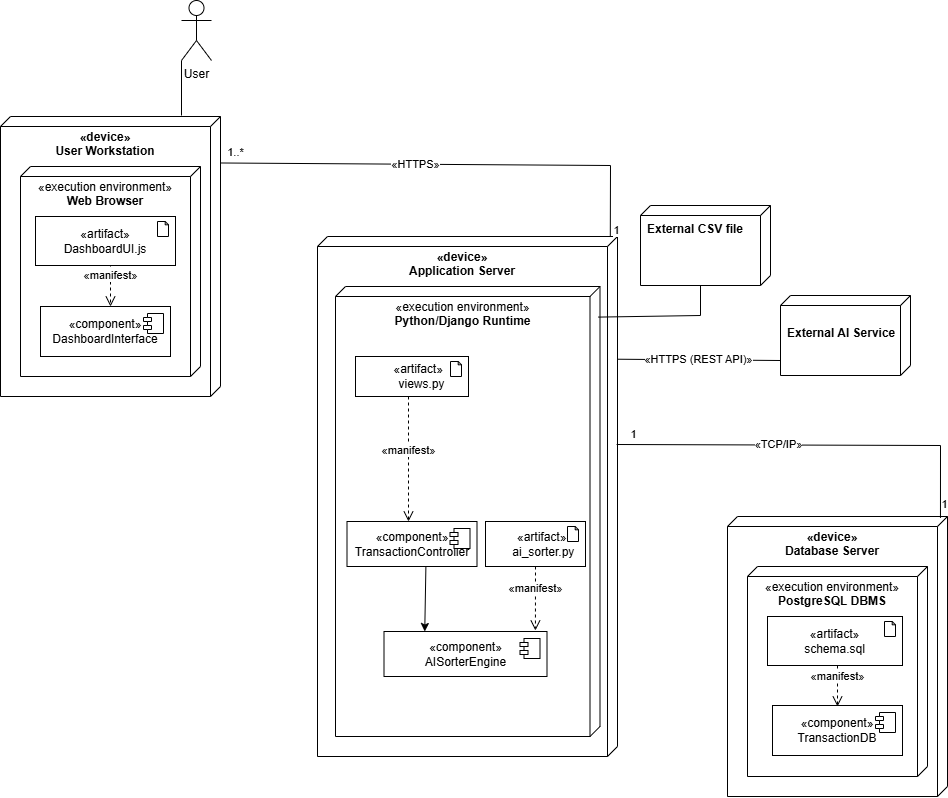
\includegraphics[width=1.0\textwidth, height=0.45\textheight, keepaspectratio]{images/deployment.png}
	\caption{System Deployment Architecture}
	\label{fig:deployment}
\end{figure}
